\documentclass{article}
\usepackage{eecstex}
\usepackage{pgfplots}

\title{EE 123 HW 02}
\author{Bryan Ngo}
\date{2022-01-29}

\begin{document}

\maketitle

\setcounter{section}{2}

\section{}

\begin{equation}
    a^n u[n] \iff \frac{1}{1 - ae^{-j \omega}}, \ |a| < 1
\end{equation}

\subsection{}

\begin{equation}
    x[n] = -b^n u[-n - 1] =
    \begin{cases}
        -b^n & n \leqslant -1 \\
        0 & n \geqslant 0
    \end{cases}
\end{equation}
Using the definition of the DTFT,
\begin{align}
    X(e^{j \omega}) &= \sum_{k \in \Z} -b^k u[-k - 1] e^{-j \omega k} \\
    &= -\sum_{k \leqslant -1} b^k e^{-j \omega k}
\end{align}
Letting \(k' = -k\),
\begin{align}
    X(e^{j \omega}) &= \sum_{k' \geqslant 1} -b^{-k'} e^{j \omega k'} \\
    &= \sum_{k \geqslant 0} -(b^{-1} e^{j \omega})^k - 1 \\
    &= 1 - \frac{1}{1 - b e^{j \omega}} \\
    &= \frac{\cancel{1} - b e^{j \omega} - \cancel{1}}{1 - b e^{j \omega}} \cdot \frac{-b e^{-j \omega}}{-b e^{-j \omega}} \\
    &= \frac{1}{1 - b e^{-j \omega}}
\end{align}
where \(|b^{-1}| < 1 \implies |b| > 1\).

\subsection{}

\begin{align}
    Y(e^{j \omega}) &= 2e^{-j \omega} \frac{1}{1 - (-2) e^{-j \omega}} \\
    \overset{\mathcal{F}^{-1}}{\implies} y[n] &= 2 (-(-2)^{n - 1} u[-(n - 1) - 1]) \\
    &= (-2)^n u[-n]
\end{align}

\newpage
\section{}

\begin{equation}
    H(z) = \frac{1 - z^{-1}}{1 - 0.25z^{-2}} = \frac{1 - z^{-1}}{(1 - 0.5z^{-1}) (1 + 0.5z^{-1})}
\end{equation}

\subsection{}

Using the \(z\)-transform multiplication property,
\begin{equation}
    Y(z) = H(z) X(z) = \frac{\cancel{1 - z^{-1}}}{(1 - 0.5z^{-1}) (1 + 0.5z^{-1}) \cancel{(1 - z^{-1})}} = \frac{1}{(1 - 0.5z^{-1}) (1 + 0.5z^{-1})}
\end{equation}
Then, using partial fraction decomposition,
\begin{align}
    Y(z) &= \frac{1}{(1 - 0.5z^{-1}) (1 + 0.5z^{-1})} = \frac{A}{1 - 0.5z^{-1}} + \frac{B}{1 + 0.5z^{-1}} \\
    &= 1 = A(1 + 0.5z^{-1}) + B(1 - 0.5z^{-1}) \\
\end{align}
Letting \(z = -0.5\), we get \(B = \frac{1}{2}\).
Letting \(z = 0.5\), we get \(A = \frac{1}{2}\).
Then,
\begin{align}
    Y(z) &= \frac{1}{2} \frac{1}{1 - 0.5z^{-1}} + \frac{1}{2} \frac{1}{1 + 0.5z^{-1}} \\
    \overset{\mathcal{Z}^{-1}}{\implies} y[n] &= \frac{1}{2} \left(\frac{1}{2}\right)^n u[n] + \frac{1}{2} \left(-\frac{1}{2}\right)^n u[n]
\end{align}

\subsection{}

\begin{equation}
    y[n] = \delta[n] - \delta[n - 1] \overset{\mathcal{Z}}{\implies} Y(z) = 1 - z^{-1} = H(z) X(z)
\end{equation}
meaning that \(X(z) = 1 - 0.25z^{-2} = (1 - 0.5z^{-1}) (1 + 0.5z^{-1})\).
By definition of the \(z\)-transform,
\begin{equation}
    x[n] = \delta[n] - \frac{1}{4} \delta[n - 2]
\end{equation}

\subsection{}

Treating the input as the real part of \(z = e^{j 0.5 \pi}\),
\begin{equation}
    H(e^{j 0.5 \pi}) = \frac{1 - e^{-j 0.5 \pi}}{1 - 0.25e^{-j\pi}} = 0.8 \sqrt{2} e^{j \frac{\pi}{4}}
\end{equation}
Meaning that the final output is
\begin{equation}
    y[n] = 0.8 \sqrt{2} \cos\left(0.5 \pi n + \frac{\pi}{4}\right)
\end{equation}

\newpage
\section{}

\begin{align}
    x[n] &= -\frac{1}{3} \left(\frac{1}{2}\right)^n u[n] - \frac{4}{3} 2^n u[-n - 1] \\
    Y(z) &= \frac{1 - z^{-2}}{\left(1 - \frac{1}{2} z^{-1}\right) (1 - 2z^{-1})}
\end{align}

\subsection{}

\begin{equation}
    X(z) = -\frac{1}{3} \frac{1}{1 - \frac{1}{2} z^{-1}} + \frac{4}{3} \frac{1}{1 - 2z^{-1}}
\end{equation}

\subsection{}

\begin{equation}
    R_y: \frac{1}{2} < |z| < 2
\end{equation}

\subsection{}

Simplifiying \(X(z)\),
\begin{align}
    X(z) &= \frac{1}{3} \frac{-(1 - 2z^{-1}) + 4 \left(1 - \frac{1}{2} z^{-1}\right)}{\left(1 - \frac{1}{2} z^{-1}\right) (1 - 2z^{-1})} \\
    &= \frac{1}{3} \frac{-1 + \cancel{2z^{-1}} + 4 - \cancel{2z^{-1}}}{\left(1 - \frac{1}{2} z^{-1}\right) (1 - 2z^{-1})} \\
    &= \frac{1}{\left(1 - \frac{1}{2} z^{-1}\right) (1 - 2z^{-1})} \\
    \implies Y(z) &= (1 - z^{-2}) X(z) = X(z) - z^{-2} X(z) \\
    \overset{\mathcal{Z}^{-1}}{\implies} y[n] &= x[n] - x[n - 2]
\end{align}

\subsection{}

\begin{equation}
    H(z) = \frac{Y(z)}{X(z)} = 1 - z^{-2} \overset{\mathcal{Z}^{-1}}{\implies} h[n] = \delta[n] - \delta[n - 2]
\end{equation}

\newpage
\section{}

\begin{align}
    X(z) &= \frac{z^{-2}}{1 - 2.3z^{-1} + 1.6z^{-2} - 0.3z^{-3}} = \frac{2.04}{1 + 0.3z^{-1}} - \frac{3.47}{1 - z^{-1}} + \frac{1.43}{(1 - z^{-1})^2} \\
    \overset{\mathcal{Z}^{-1}}{\implies} x[n] &= (-0.3)^n u[n] - 3.47 u[n] + 1.43 (n + 1) u[n + 1]
\end{align}

\newpage
\section{}

\begin{enumerate}
    \item System A, causal, stable, ROC: \(|z| > 0.9\)
    \item System B, non-causal, stable, ROC: \(|z| < 1.111\)
    \item System A, non-causal, unstable, ROC: \(|z| < 0.9\)
\end{enumerate}

\newpage
\section{}

\begin{equation}
    Z(e^{j \omega}) = \frac{1}{2\pi} \int_{-\pi}^\pi X(e^{j \theta}) Y(e^{j (\omega - \theta)}) \, d\theta
\end{equation}

\subsection{}

\begin{align}
    Y(e^{j \omega}) &= \pi \sum_{k = -\infty}^\infty \delta(\omega - \pi + 2\pi k) + \delta(\omega + \pi + 2\pi k) \\
    X(e^{j \omega}) \ast Y(e^{j \omega}) &= \frac{1}{2} \int_{-\pi}^\pi X(e^{j \theta}) \sum_{k \in \Z} \delta((\omega - \theta) - \pi + 2\pi k) + \delta((\omega - \theta) + \pi + 2\pi k) \, d\theta \\
    &= \frac{1}{2} \sum_{k \in \Z} \int_{-\pi}^\pi X(e^{j \omega}) (\delta(\omega - \theta - \pi + 2\pi k) + \delta(\omega + \theta + \pi + 2\pi k)) \, d\theta \\
    &= \frac{1}{2} \sum_{k \in \Z} (X(e^{j (\omega - \pi + 2\pi k)}) + X(e^{j (\omega + \pi + 2\pi k)}))
\end{align}
\begin{center}
    \begin{tikzpicture}
        \begin{axis}[
            xlabel={\(\frac{\omega}{\pi}\)}, ylabel={\(Z(e^{j \omega})\)},
            title={DTFT of Product},
            axis lines=middle,
        ]
        \addplot[color=blue] table[
            col sep=comma,
            x=index, y=8a
        ]{q8.csv};
        \end{axis}
    \end{tikzpicture}
\end{center}

\subsection{}

\begin{align}
    Y(e^{j \omega}) &= \pi \sum_{k = -\infty}^\infty \delta\left(\omega - \frac{\pi}{2} + 2\pi k\right) + \delta\left(\omega + \frac{\pi}{2} + 2\pi k\right) \\
    X(e^{j \omega}) \ast Y(e^{j \omega}) &= \frac{1}{2} \sum_{k \in \Z} \left(X\left(e^{j \left(\omega - \frac{\pi}{2} + 2\pi k\right)}\right) + X\left(e^{j \left(\omega + \frac{\pi}{2} + 2\pi k\right)}\right)\right)
\end{align}
\begin{center}
    \begin{tikzpicture}
        \begin{axis}[
            xlabel={\(\frac{\omega}{\pi}\)}, ylabel={\(Z(e^{j \omega})\)},
            title={DTFT of Product},
            axis lines=middle,
        ]
        \addplot[color=blue] table[
            col sep=comma,
            x=index, y=8b
        ]{q8.csv};
        \end{axis}
    \end{tikzpicture}
\end{center}

\subsection{}

\begin{align}
    Y(e^{j \omega}) &= \pi \sum_{k = -\infty}^\infty \delta\left(\omega - \frac{\pi}{4} + 2\pi k\right) + \delta\left(\omega + \frac{\pi}{4} + 2\pi k\right) + \delta\left(\omega - \frac{3\pi}{4} + 2\pi k\right) + \delta\left(\omega + \frac{3\pi}{4} + 2\pi k\right) \\
    X(e^{j \omega}) \ast Y(e^{j \omega}) &= \frac{1}{2} \sum_{k \in \Z} \left(X\left(e^{j \left(\omega - \frac{\pi}{2} + 2\pi k\right)}\right) + X\left(e^{j \left(\omega + \frac{\pi}{2} + 2\pi k\right)}\right)\right)
\end{align}
\begin{center}
    \begin{tikzpicture}
        \begin{axis}[
            xlabel={\(\frac{\omega}{\pi}\)}, ylabel={\(Z(e^{j \omega})\)},
            title={DTFT of Product},
            axis lines=middle,
        ]
        \addplot[color=blue] table[
            col sep=comma,
            x=index, y=8c
        ]{q8c.csv};
        \end{axis}
    \end{tikzpicture}
\end{center}

\subsection{}

\begin{align}
    Y(e^{j \omega}) &= \pi \sum_{k = -\infty}^\infty \cancelto{1}{e^{j \frac{\pi}{2}}} \delta(\omega - \pi + 2\pi k) + \cancelto{-1}{e^{-j \frac{\pi}{2}}} \delta(\omega + \pi + 2\pi k) \\
    X(e^{j \omega}) \ast Y(e^{j \omega}) &= \frac{1}{2} \sum_{k \in \Z} (X(e^{j (\omega - \pi + 2\pi k)}) - X(e^{j (\omega + \pi + 2\pi k)}))
\end{align}
\begin{center}
    \begin{tikzpicture}
        \begin{axis}[
            xlabel={\(\frac{\omega}{\pi}\)}, ylabel={\(Z(e^{j \omega})\)},
            title={DTFT of Product},
            axis lines=middle,
        ]
        \addplot[color=blue] table[
            col sep=comma,
            x=index, y=8d
        ]{q8.csv};
        \end{axis}
    \end{tikzpicture}
\end{center}

\newpage
\section{}

\begin{equation}
    H(e^{j \omega}) =
    \begin{cases}
        j & \omega \in (-\pi, 0) \\
        0 & \omega = 0 \\
        -j & \omega \in (0, \pi)
    \end{cases}
\end{equation}

\subsection{}

From Table 2.1 of O\&S, the symmetry properties of the DTFT imply that the Hilbert filter impulse response is purely \emph{real and odd}.

\subsection{}

\begin{align}
    X(e^{j \omega}) &= \pi (\delta(\omega - \omega_0) + \delta(\omega + \omega_0)) \\
    Y(e^{j \omega}) &= -j \pi (\delta(\omega - \omega_0) - \delta(\omega + \omega_0)) \\
    \overset{\mathcal{F}^{-1}}{\implies} y[n] &= \sin(\omega_0 n)
\end{align}

\subsection{}

\begin{align}
    Y(e^{j \omega}) &= H(e^{j \omega})^2 X(e^{j \omega}) =
    \begin{cases}
        -X(e^{j \omega}) & \omega \in (-\pi, 0) \\
        0 & \omega = 0 \\
        -X(e^{j \omega}) & \omega \in (0, \pi)
    \end{cases} \\
    &= -X(e^{j \omega}) \overset{\mathcal{F}^{-1}}{\implies} y[n] = -x[n]
\end{align}

\subsection{}

\begin{center}
    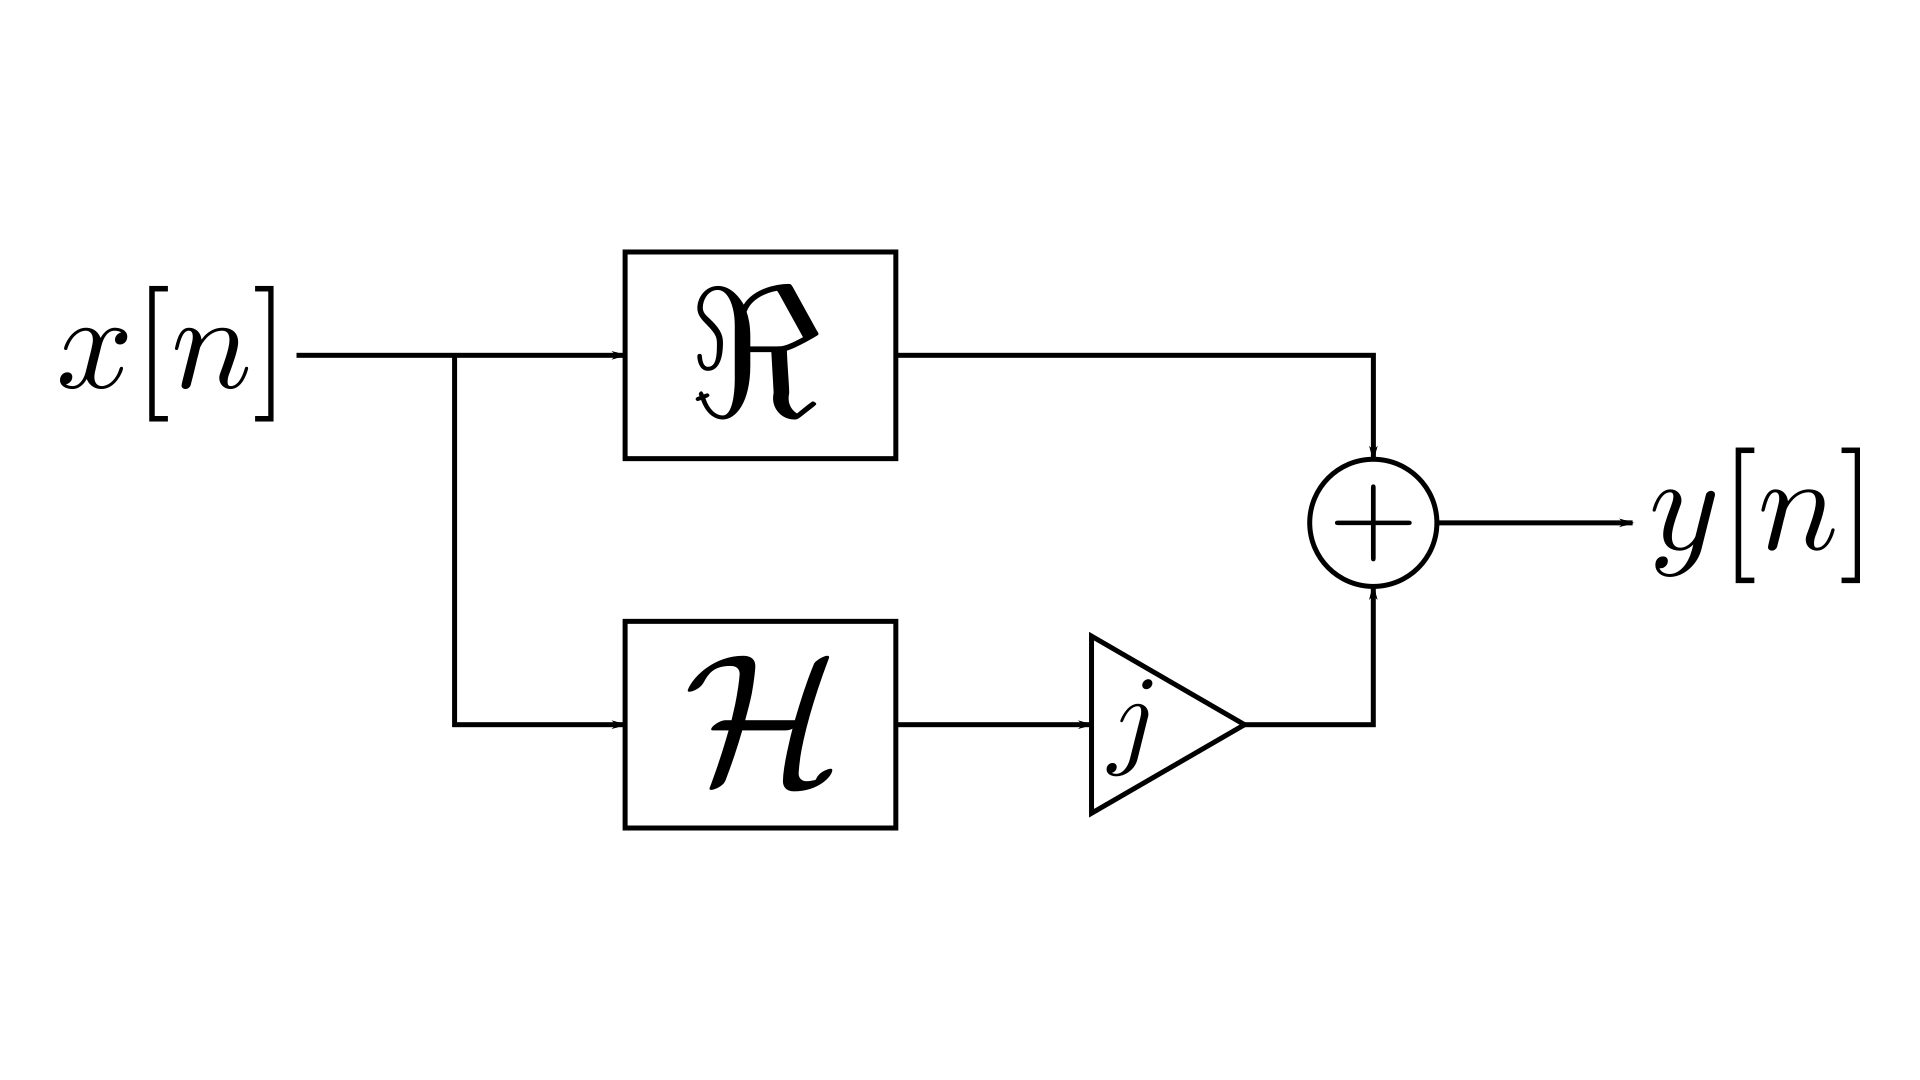
\includegraphics[width=0.6\textwidth]{q9d.png}
\end{center}
where \(\mathcal{H}\) is the Hilbert transform.

\end{document}
